\documentclass[simplex.tex]{subfiles}
% NO NEED TO INPUT PREAMBLES HERE
% packages are inherited; you can compile this on its own
\begin{document}
\subsection{Robust Law of Large Graphs}
Your content here. Please make sure that it fits on one page.

%%%   EXAMPLE FIGURE BLOCK
\begin{figure}[!h]
\begin{cframed}
\centering

\includegraphics[width=0.15\textwidth]{neurodata_small.png}
\caption{Please provide a detailed caption for your figure.}
\label{fig:name}
\end{cframed}
\end{figure}
%
%To estimate the mean of a collection of weighted graphs under a
%low rank random graph model (e.g. Stochastic Blockmodel) when
%observing contaminated graphs, we propose an estimator which not
%only inherits robustness from element-wise robust estimators but
%also has small variance due to application of a rank-reduction
%procedure. Under appropriate conditions, we prove that our
%estimator outperforms standard estimators via asymptotic relative
%efficiency.  Previously we illustrated our theory and methods by Monte
%Carlo simulation. And now we focus on the real data experiment.
%
%
%The real data we consider is a structural connectomic data.
%The graphs are based on diffusion tensor MR
%images. It contains 114 different brain scans, each of
%which was processed to yield an undirected, weighted graph with no
%self-loops, using the m2g/ndmg pipelines.  The vertices of the graphs
%represent different regions in the brain defined according to an atlas.
%We used the  desikan atlas with 70 vertices. The weight of an edge
%between two vertices represents the number of white-matter tract
%connecting the corresponding two regions of the brain.
%As we know, ndmg is a better pipeline compared to m2g, which means that the mean graph derived from ndmg should be a more accurate estimate to actual population mean graph.
%In order to evaluate the performance of the four estimators, we build estimates based on the samples from m2g, while using the sample mean graph from ndmg as an estimate of the probability matrix $P$.
%Specifically, each Monte Carlo replicate corresponds to sampling $m$ graphs out
%of the 114 from the m2g dataset and computing the four estimates based on the $m$ sampled graphs.
%We then compared these estimates to the sample mean for the 114 graphs from the ndmg dataset.
%We ran 100 simulations for the sample sizes $m=2, 5, 10$.
%We also considered all possible dimensions for adjacency spectral embedding by ranging d from 1 to 70 in
%order to investigate the impact of the dimension selection procedures.
%We plot the result in figure~\ref{fig:robDim}
%
%
%
%\begin{figure}[h!]
%\begin{cframed}
%\centering
%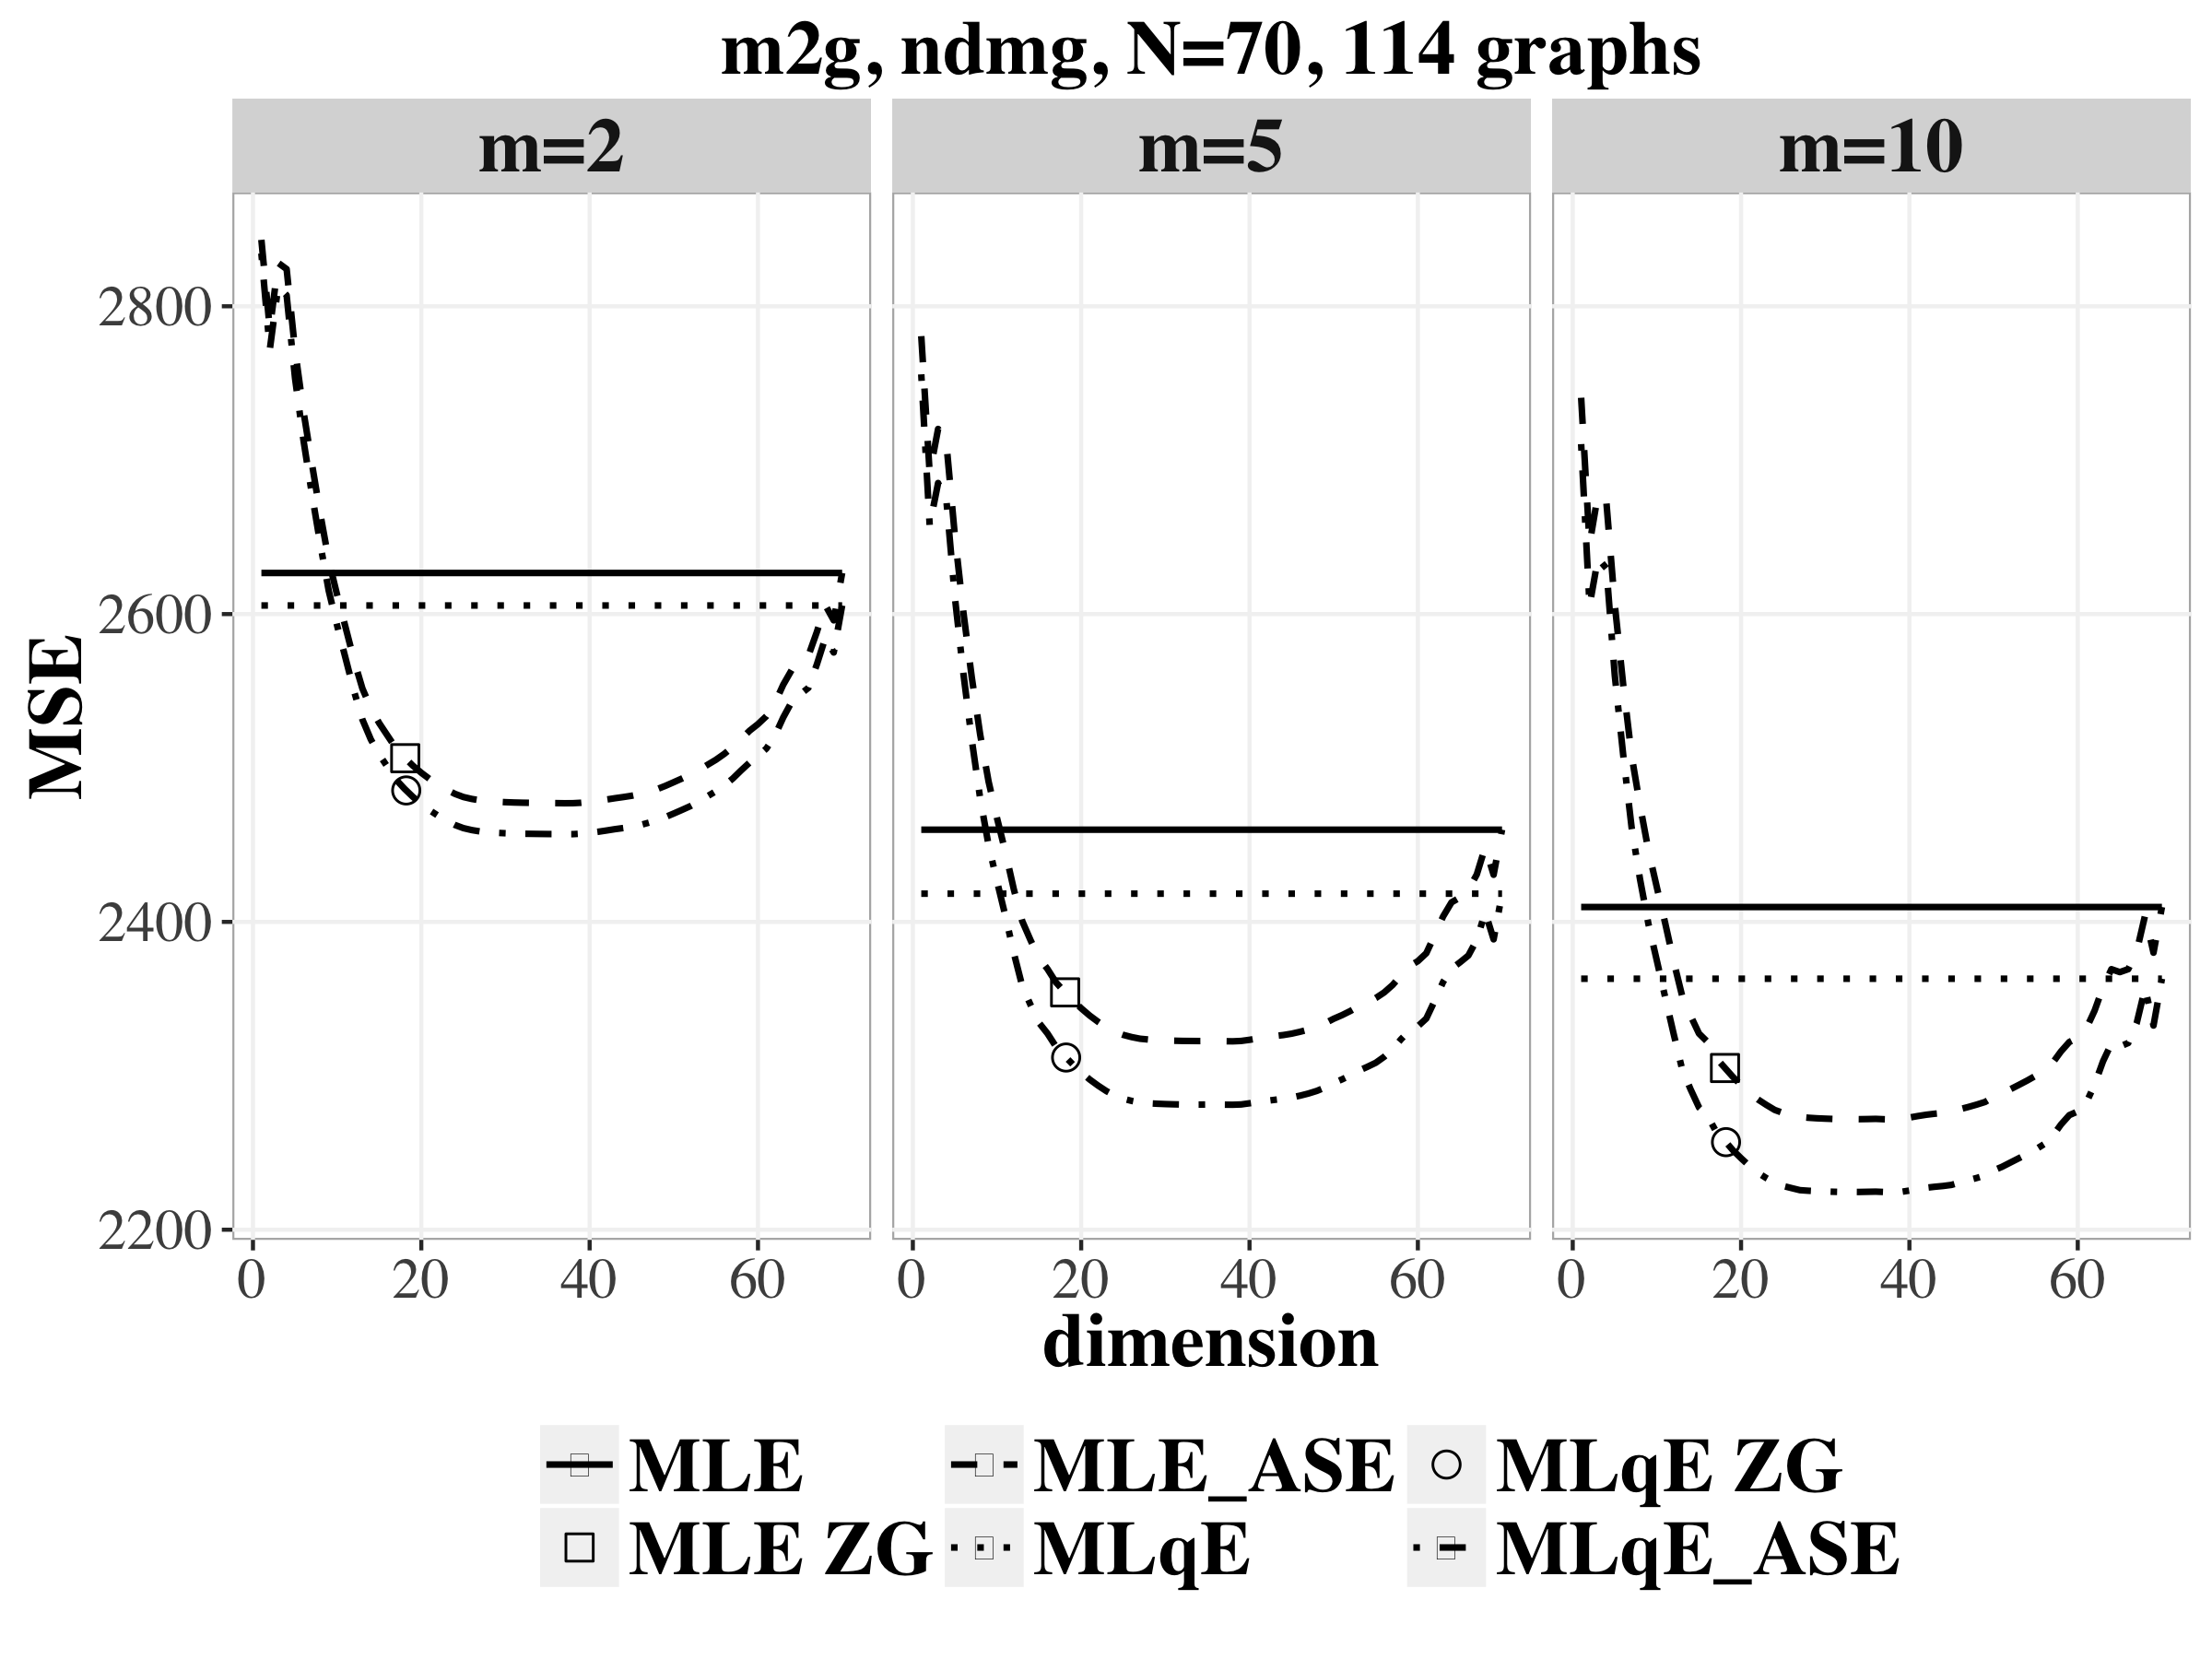
\includegraphics[width=\textwidth]{../../figs/CCI_m2g_ndmg_Weighted_q_0.9_EIG.png}
%\caption{
%{\bf Comparison of MSE of the four estimators for the desikan atlases at three sample sizes based on m2g and ndmg pipelines.}  
%{\bf 1. MLE (horizontal solid line) vs MLqE (horizontal dotted line):} 
%ML$q$E outperforms MLE since robust estimators are always preferred in practice;
%{\bf 2. MLE (horizontal solid line) vs MLE\_ASE (dashed line):} MLE\_ASE wins the bias-variance tradeoff when embedded into a proper dimension; 
%{\bf 3. MLqE (horizontal dotted line) vs ML$q$E\_ASE (dashed dotted line):}
%ML$q$E\_ASE wins the bias-variance tradeoff when embedded into a proper dimension; 
%{\bf 4.  ML$q$E\_ASE (dashed dotted line) vs MLE\_ASE (dashed
%line):}
%MLqE\_ASE is better, since it inherits the robustness from 
%ML$q$E. And the square and circle represent the dimensions selected by the Zhu and Ghodsi method. We can see it does a pretty good job. But more importantly, a wide range of dimensions could lead to an improvement.
%}
%\label{fig:robDim}
%\end{cframed}
%\end{figure}
%
%
%
\end{document}
